\documentclass{beamer}
\usetheme{default}
\usepackage{graphicx}



\begin{document}
\begin{frame}{Angular Correlation Function}
	$$F = 1 + a \frac{\boldsymbol{p_e}\cdot\boldsymbol{p_\nu}}{E_eE_\nu} + b \frac{m_e}{E} + c \left(\frac{\boldsymbol{p_e}\cdot\boldsymbol{p_\nu}}{3E_eE_\nu}-\frac{(\boldsymbol{p_e}\cdot\boldsymbol{j})(\boldsymbol{p_\nu}\cdot\boldsymbol{j})}{E_eE_\nu}\right) $$$$+ \frac{\boldsymbol{J}}J\cdot\left(A \frac{\boldsymbol{p_e}}{E_e} + B \frac{\boldsymbol{p_\nu}}{E_\nu} + D \frac{\boldsymbol{p_e}\times\boldsymbol{p_\nu}}{E_eE_\nu}\right)$$
	Spherical Coordinates ($\boldsymbol{J}$ parallel to positive Z axis)
	$$\boldsymbol{\beta_e} = (r=\beta_e;\theta=\theta_e;\phi=0),\;\cos(\theta_e) \equiv z_e,\;\beta_e = \frac{|\boldsymbol{p_e}|}{E} = \sqrt{1-\frac{m_e^2}{E^2}}$$
	$$\boldsymbol{\beta_\nu} = (r=1;\theta=\theta_\nu;\phi=\phi),\quad\cos(\theta_\nu) \equiv z_\nu$$
	$$\boldsymbol{\beta_e}\cdot\boldsymbol{\beta_\nu} = \beta_e(\cos\theta_e\cos\theta_\nu + \sin\theta_e\sin\theta_\nu\cos\phi) =$$
	$$ \beta_e(z_ez_\nu + \sqrt{1-z^2_e}\sqrt{1-z^2_\nu}\cos\phi)$$
	$$\boldsymbol{\beta_e}\cdot\boldsymbol{j} = \beta_e\cos\theta_e=\beta_ez_e$$
	$$\boldsymbol{\beta_\nu}\cdot\boldsymbol{j} = \cos\theta_\nu=z_\nu$$
	$$\boldsymbol{j}\cdot(\boldsymbol{\beta_e}\times\boldsymbol{\beta_\nu})=\beta_e\sin\theta_e\sin\theta_\nu\sin\phi=\beta_e\sqrt{1-z^2_e}\sqrt{1-z^2_\nu}\sin\phi$$
\end{frame}	
\begin{frame}{Angular Correlation Factor}
	$$(\boldsymbol{\beta_e}\cdot\boldsymbol{j})(\boldsymbol{\beta_\nu}\cdot\boldsymbol{j}) = z_ez_\nu$$
	Putting all together:
	$$F = 1 + a\beta(z_ez_\nu+\sqrt{1-z_e^2}\sqrt{1-z_\nu^2}\cos\phi) + b\frac {m_e}E +$$
	$$+c\beta\left(-\frac{2}{3}z_ez_\nu+\frac{1}{3}\sqrt{1-z_e^2}\sqrt{1-z_\nu^2}\right)+A\beta z_e+ Bz_\nu+$$
	$$+D\beta\sqrt{1-z_e^2}\sqrt{1-z_\nu^2}\sin\phi =$$
	$$ = 1 + b\frac {m_e}E + \left(a-\frac 23 c\right)\beta z_ez_\nu+ A\beta z_e + Bz_\nu +$$
	$$ + \beta \sqrt{1-z_e^2}\sqrt{1-z_\nu^2} \left(\left(a+\frac c3\right)\cos\phi + D \sin\phi\right)$$
\end{frame}


\begin{frame}{Single Variable: c}{Angular Correlation Factor}
	\begin{figure}
		\centering
		\includegraphics[width=0.4\paperwidth]{plots/c_3D_image.png}
		\includegraphics[width=0.4\paperwidth]{plots/c_max_min.png}
		\caption{(Right) Values of the angular correlation Factor with a = 1, E = 5000 keV and rest of variables 0. (Left) Location of maximum (blue, value = 1.995) and minimum (orange, value = 0.005)}	
	\end{figure}
\end{frame}
\begin{frame}{Single Variable: c}{Angular Correlation Factor}
	\begin{figure}
		\centering
		\includegraphics[width=0.8\paperwidth]{plots/crosssections_c.png}
		\caption{(Right) 2D projection of previous 3D image at $\phi = 0$ (Left) 1D projections at $\phi=0$, and either $z_\nu = 0$ or $z_\nu = 1$}
	\end{figure}
\end{frame}
\begin{frame}{Single Variable c}{Sampling}
	\begin{figure}
		\centering
		\includegraphics[height=.8\textheight]{plots/sample_cpairplot}
		\caption{Pair plots for N = 100000 decays with c = 1, E = 1000 keV}
	\end{figure}
\end{frame}
\begin{frame}{Single Variable c}{Marginal distributions}

	
	For $z_e$ (and $z_\nu$ by symmetry of the expresions), we can observe reason why the marginal distribution becomes constant: 
	
	$$f(z_e) = N\int_{-1}^{1}dz_\nu\int_{0}^{2\pi}d\phi F =$$$$= N\int_{-1}^{1}dz_\nu\int_{0}^{2\pi}d\phi \left(1 + c\beta\left(-\frac 23 z_ez_\nu+\frac 13 \sqrt{1-z^2_e}\sqrt{1-z^2_\nu}\cos \phi\right)\right) $$$$ = N\int_{-1}^{1}dz_\nu\int_{0}^{2\pi}d\phi = 4\pi N = N $$

	
\end{frame}
\begin{frame}{Single Variable a}{Marginal distributions}
	
	
	For $\phi$, we can derive the expected shape: 
	
	$$f(\phi) = N\int_{-1}^{1}dz_\nu\int_{-1}^{1}dz_e F $$$$= N\int_{-1}^{1}dz_\nu\int_{-1}^{1}dz_e \left(1 + c\beta\left(-\frac 23 z_ez_\nu+\frac 13 \sqrt{1-z^2_e}\sqrt{1-z^2_\nu}\cos \phi\right)\right)$$$$ = N\left(4+a\beta\left(\frac{\pi}{2}\right)^2\cos\phi/3\right) = N\left(1+a\beta\frac{\pi^2}{48}\cos\phi\right)  $$
	
	
\end{frame}
\begin{frame}{Single Variable a}{Marginal distributions}
	
	\begin{figure}
		\centering
		\includegraphics[height=0.7\textheight]{plots/hist_c_phi}
		\caption{Histogram showing the values of $\phi$ with a = 1, E = 1000 keV for N = 100000 decays, and curve showing the theoretical distribution}
	\end{figure}
\end{frame}
\begin{frame}{Two variables: c and B}
	Since term proportional to a depends on E, we can consider different ratios by either:
	\begin{itemize}
		\item Fixing $c = B = 1$ and modifying the energy
		\item Same as before, but now $B = -1$
		\item Fixing $B = 1$ and $E \gg m_e \rightarrow \beta_e \approx 1$ and modifying $c > B$
	\end{itemize}
	
	We recall
	
	$$F = 1 + c\beta_e\left(-\frac 23 z_ez_\nu + \frac 13 \sqrt{1-z^2_e}\sqrt{1-z^2_\nu}\cos \phi\right) + Bz_\nu$$
	
	Maxima and minima with $z_e=\pm1,z_\nu \pm1 \rightarrow \boldsymbol{p_e} \parallel \boldsymbol{p_\nu} \parallel \boldsymbol{J}$  
	
\end{frame}
\begin{frame}{Two variables: c and B}{Angular Correlation Factor}
	\begin{figure}
		\centering
		\includegraphics[width=0.4\paperwidth]{plots/posc_posB_lowE_3D}
		\includegraphics[width=0.4\paperwidth]{plots/posc_negB_lowE_3D}
		\caption{Values of the angular correlation Factor with (Right) c = 1, B = 1 and (Left) c = 1, B = -1; with E = 520 keV and rest of variables 0 for both.}
	\end{figure}
\end{frame}
\begin{frame}{Two variables: c and B}{Angular Correlation Factor}
	\begin{figure}
		\centering
		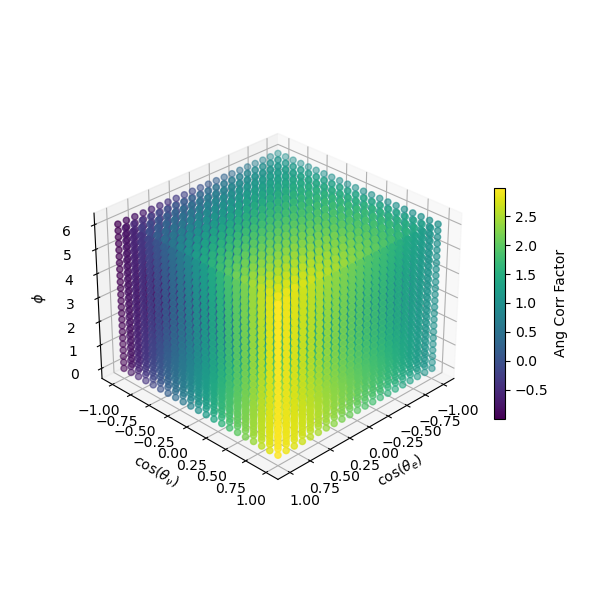
\includegraphics[width=0.4\paperwidth]{plots/posa_posB_hiE_3D}
		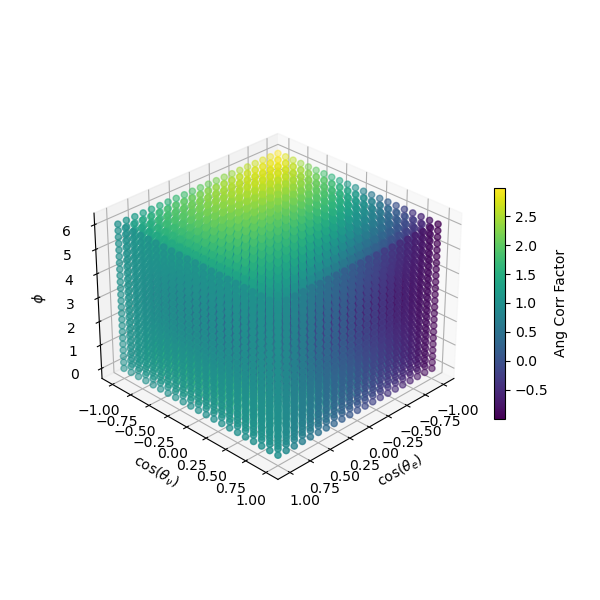
\includegraphics[width=0.4\paperwidth]{plots/posa_negB_hiE_3D}
		\caption{Values of the angular correlation Factor with (Right) c = 1, B = 1 and (Left) c = 1, B = -1; with E = 5000 keV and rest of variables 0 for both.}
	\end{figure}
\end{frame}
\begin{frame}{Two variables: c and B}{Angular Correlation Factor}
	\begin{figure}
		\centering
		\includegraphics[width=0.4\paperwidth]{plots/posc_posB_medE_3D}
		\includegraphics[width=0.4\paperwidth]{plots/posc_posB_vhic_3D}
		\caption{Values of the angular correlation Factor with (Right) a = c, B = 1, E = 800 keV and (Left) c = 5, B = 1, E = 5000 keV; with the rest of variables 0 for both.}
	\end{figure}
\end{frame}
\begin{frame}{Two variables: c and B}{Maximum and Minimum}
	\begin{figure}
		\centering
		\includegraphics[width=0.4\paperwidth]{plots/posc_posB_hiE_max_min}
		\includegraphics[width=0.4\paperwidth]{plots/posc_negB_hiE_max_min}
		\caption{Location of maximum (blue, value = 2.66318) and minimum (orange, value = -0.66318) for (Right) c = B = 1, E = 5000 keV and (Left) c = 1, B = -1, E = 5000 keV}
	\end{figure}
\end{frame}
\begin{frame}{Two variable: c and B}{Sampling}
	\begin{figure}
		\centering
		\includegraphics[height=0.6\textheight]{plots/sample_posc_posB_hiE_pairplot}
		\caption{Pairplot with the marginal distributions for a simulation of N = 300000 decays with c = B = 1, E = 5000 keV. The 1 variable histograms show the theoretical distribution obtained from numerically integrating F with the constrain $F > 0$}
	\end{figure}
\end{frame}
\begin{frame}{Two variables: c and A}
	Since both terms proportional to a depends on E, we can consider only consider different ratios by changing one ($c$), while leaving the other ($A$) fixed. For convenience $E \gg m_e$.
	
	$$F = 1 + \beta_e\left(c \left(-\frac 23 z_ez_\nu + \frac 13 \sqrt{1-z^2_e}\sqrt{1-z^2_\nu}\cos \phi\right) + Az_e\right)$$
	
	Maximum and minimum with $z_e=\pm1,z_\nu \pm1 \rightarrow \boldsymbol{p_e} \parallel \boldsymbol{p_\nu} \parallel \boldsymbol{J}$  
	
\end{frame}
\begin{frame}{Two variables: c and A}{Angular Correlation Factor}
	\begin{figure}
		\centering
		\includegraphics[width=0.4\paperwidth]{plots/posA_xsposc_3D}
		\includegraphics[width=0.4\paperwidth]{plots/posA_xsnegc_3D}
		\caption{Values of the angular correlation Factor with (Right) A = 1, c = 0.25 and (Left) A = 1, c = -0.25, with E = 100000 keV and rest of variables 0 for both.}
	\end{figure}
\end{frame}
\begin{frame}{Two variables: c and A}{Angular Correlation Factor}
	\begin{figure}
		\centering
		\includegraphics[width=0.4\paperwidth]{plots/posA_eqposc_3D}
		\includegraphics[width=0.4\paperwidth]{plots/posA_eqnegc_3D}
		\caption{Values of the angular correlation Factor with (Right) A = 1, c = 1 and (Left) A = 1, c = -1, with E = 100000 keV and rest of variables 0 for both.}
	\end{figure}
\end{frame}
\begin{frame}{Two variables: c and A}{Angular Correlation Factor}
	\begin{figure}
		\centering
		\includegraphics[width=0.4\paperwidth]{plots/posA_xlposc_3D}
		\includegraphics[width=0.4\paperwidth]{plots/posA_xlnegc_3D}
		\caption{Values of the angular correlation Factor with (Right) A = 1, c = 4 and (Left) A = 1, c = -4, with E = 100000 keV and rest of variables 0 for both.}
		
	\end{figure}
\end{frame}
\begin{frame}{Two variables: c and A}{Maximum and Minimum}
	\begin{figure}
		\centering
		\includegraphics[width=0.4\paperwidth]{plots/posA_eqposc_max_min}
		\includegraphics[width=0.4\paperwidth]{plots/posA_eqnegc_max_min}
		\caption{Location of maximum (blue, value = 2.66664) and minimum (orange, value = -0.66664) for (Right) A = c = 1, E = 100000 keV and (Left) A = 1, c = -1, E = 100000 keV}
	\end{figure}
\end{frame}
\begin{frame}{Two variable: c and A}{Sampling}
	\begin{figure}
		\centering
		\includegraphics[height=0.6\textheight]{plots/sample_cA_eqpos_pairplot}
		\caption{Pairplot with the marginal distributions for a simulation of N = 300000 decays with c = A = 1, E = 100000 keV. The 1 variable histograms show the theoretical distribution obtained from numerically integrating F with the constrain $F > 0$}
	\end{figure}
\end{frame}
\begin{frame}{Two variables: c and a}
	Since both terms proportional to a depends on E, we can consider only consider different ratios by changing one ($c$), while leaving the other ($A$) fixed. For convenience $E \gg m_e$.
	
	$$ F = 1 +\left(a-\frac 23 c\right)\beta z_ez_\nu + \beta \sqrt{1-z_e^2}\sqrt{1-z_\nu^2} \left(a+\frac c3\right)\cos\phi $$
	
	Maximum and minimum depends on the relative signs of a and c
	\begin{itemize}
		\item c and a opposite sign: $z_e = \pm1,z_\nu = \pm1 \rightarrow \boldsymbol{p_e} \parallel \boldsymbol{p_\nu} \parallel \boldsymbol{J}$
		\item c and a same sign: $z_e = 0,z_\nu = 0 \rightarrow \boldsymbol{p_e} \parallel \boldsymbol{p_\nu} \perp \boldsymbol{J}$    
	\end{itemize} 
	
\end{frame}
\begin{frame}{Two variables: c and a}{Angular Correlation Factor}
	\begin{figure}
		\centering
		\includegraphics[width=0.4\paperwidth]{plots/posa_xsposc_3D}
		\includegraphics[width=0.4\paperwidth]{plots/posa_xsnegc_3D}
		\caption{Values of the angular correlation Factor with (Right) a = 1, c = 0.25 and (Left) a = 1, c = -0.25, with E = 100000 keV and rest of variables 0 for both.}
	\end{figure}
\end{frame}
\begin{frame}{Two variables: c and A}{Angular Correlation Factor}
	\begin{figure}
		\centering
		\includegraphics[width=0.4\paperwidth]{plots/posa_eqposc_3D}
		\includegraphics[width=0.4\paperwidth]{plots/posa_eqnegc_3D}
		\caption{Values of the angular correlation Factor with (Right) a = 1, c = 1 and (Left) a = 1, c = -1, with E = 100000 keV and rest of variables 0 for both.}
	\end{figure}
\end{frame}
\begin{frame}{Two variables: c and A}{Angular Correlation Factor}
	\begin{figure}
		\centering
		\includegraphics[width=0.4\paperwidth]{plots/posa_xlposc_3D}
		\includegraphics[width=0.4\paperwidth]{plots/posa_xlnegc_3D}
		\caption{Values of the angular correlation Factor with (Right) a = 1, c = 4 and (Left) a = 1, c = -4, with E = 100000 keV and rest of variables 0 for both.}
		
	\end{figure}
\end{frame}
\begin{frame}{Two variables: c and a}{Maximum and Minimum}
	\begin{figure}
		\centering
		\includegraphics[width=0.4\paperwidth]{plots/posa_eqposc_max_min}
		\includegraphics[width=0.4\paperwidth]{plots/posa_eqnegc_max_min}
		\caption{Location of maximum (blue) and minimum (orange) for (Right) a = c = 1, E = 100000 keV (values 2.33332, -0.33332) and (Left) a = 1, c = -1, E = 100000 keV (values 2.66664, -0.66664)}
	\end{figure}
\end{frame}
\begin{frame}{Two variable: c and a}{Sampling}
	\begin{figure}
		\centering
		\includegraphics[height=0.55\textheight]{plots/sample_ac_eqpos_pairplot}
		\caption{Pairplot with the marginal distributions for a simulation of N = 300000 decays with c = a = 1, E = 100000 keV. The 1 variable histograms show the theoretical distribution obtained from numerically integrating F with the constrain $F > 0$}
	\end{figure}
\end{frame}
\begin{frame}{Two variables: c and D}{Angular Correlation Factor}
	Since both terms proportional to a depends on E, we can consider only consider different ratios by changing one ($c$), while leaving the other ($D$) fixed. For convenience $E \gg m_e$.
	
	$$F = 1 + \beta_e\left(-\frac 23 c z_ez_\nu + \left(\frac 13 c\cos\phi + D \sin  \phi\right) \sqrt{1-z^2_e}\sqrt{1-z^2_\nu}\right)$$
	
	Maxima and minima depend on the ratio between D and c:
	\begin{itemize}
		\item If $c^2 < 3D^2$: maximum at $z_e = z_\nu = 0$ and	
		$$\tan\phi = \frac {3D}c$$
		$$F = 1 + \beta_e\sqrt{D^2+\left(\frac c3\right)^2}$$ 
	\end{itemize}
\end{frame}
\begin{frame}{Two variables: c and D}{Angular Correlation Factor}
	Since both terms proportional to a depends on E, we can consider only consider different ratios by changing one ($c$), while leaving the other ($D$) fixed. For convenience $E \gg m_e$.
	
	$$F = 1 + \beta_e\left(-\frac 23 c z_ez_\nu + \left(\frac 13 c\cos\phi + D \sin  \phi\right) \sqrt{1-z^2_e}\sqrt{1-z^2_\nu}\right)$$
	
	Maxima and minima depend on the ratio between D and c:
	\begin{itemize}
		\item If $c^2 > 3D^2$: maximum at $z_e = z_\nu =\pm 1$ and	
		$$F = 1 + \frac{2}{3}\beta|c|$$ 
	\end{itemize}
	We look only at properties of the extrema
\end{frame}
\begin{frame}{Two variables: c and D}{Maximum and Minimum}
	\begin{figure}
		\centering
		\includegraphics[width=0.4\paperwidth]{plots/posD_xsposc_max_min}
		\includegraphics[width=0.4\paperwidth]{plots/posD_xsnegc_max_min}
		\caption{Positions of the maximum and minimum with Factor with (Right) D = 1, c = 0.25 and (Left) D = 1, c = -0.25, with E = 100000 keV and rest of variables 0 for both.}
	\end{figure}
\end{frame}
\begin{frame}{Two variables: c and D}{Maximum and Minimum}
	\begin{figure}
		\centering
		\includegraphics[width=0.4\paperwidth]{plots/posD_eqposc_max_min}
		\includegraphics[width=0.4\paperwidth]{plots/posD_eqnegc_max_min}
		\caption{Positions of the maximum and minimum with with (Right) D = 1, c = 1 and (Left) D = 1, c = -1, with E = 100000 keV and rest of variables 0 for both.}
	\end{figure}
\end{frame}
\begin{frame}{Two variables: c and D}{Maximum and Minimum}
	\begin{figure}
		\centering
		\includegraphics[width=0.4\paperwidth]{plots/posD_lposc_max_min}
		\includegraphics[width=0.4\paperwidth]{plots/posD_lnegc_max_min}
		\caption{Positions of the maximum and minimum with (Right) D = 1, c = 2 and (Left) D = 1, c = -2, with E = 100000 keV and rest of variables 0 for both.}
	\end{figure}
\end{frame}
\begin{frame}{Two variables: c and D}{Behaviour of maximum}
	\begin{figure}
		\centering
		\includegraphics[width=0.8\paperwidth]{plots/cD_max_behaviour}
		\caption{Behaviour of the $\phi$ coordinate for the maximum and the maximum value of the angular correlation factor for diferent values of c. Note discrepancies are a result of a sampling too coarse.}
	\end{figure}
\end{frame}

\begin{frame}{Two variable: c and D}{Sampling}
	\begin{figure}
		\centering
		\includegraphics[height=0.6\textheight]{plots/sample_cD_eqpos_pairplot}
		\caption{Pairplot with the marginal distributions for a simulation of N = 300000 decays with c = D = 1, E = 100000 keV. The 1 variable histograms show the theoretical distribution obtained from numerically integrating F with the constrain $F > 0$}
	\end{figure}
\end{frame}
\end{document}
